\chapter{Electroweak theory in the Standard Model of particles}\label{cap:introduccion}
\section{Introduction}
\begin{figure}
    \centering
    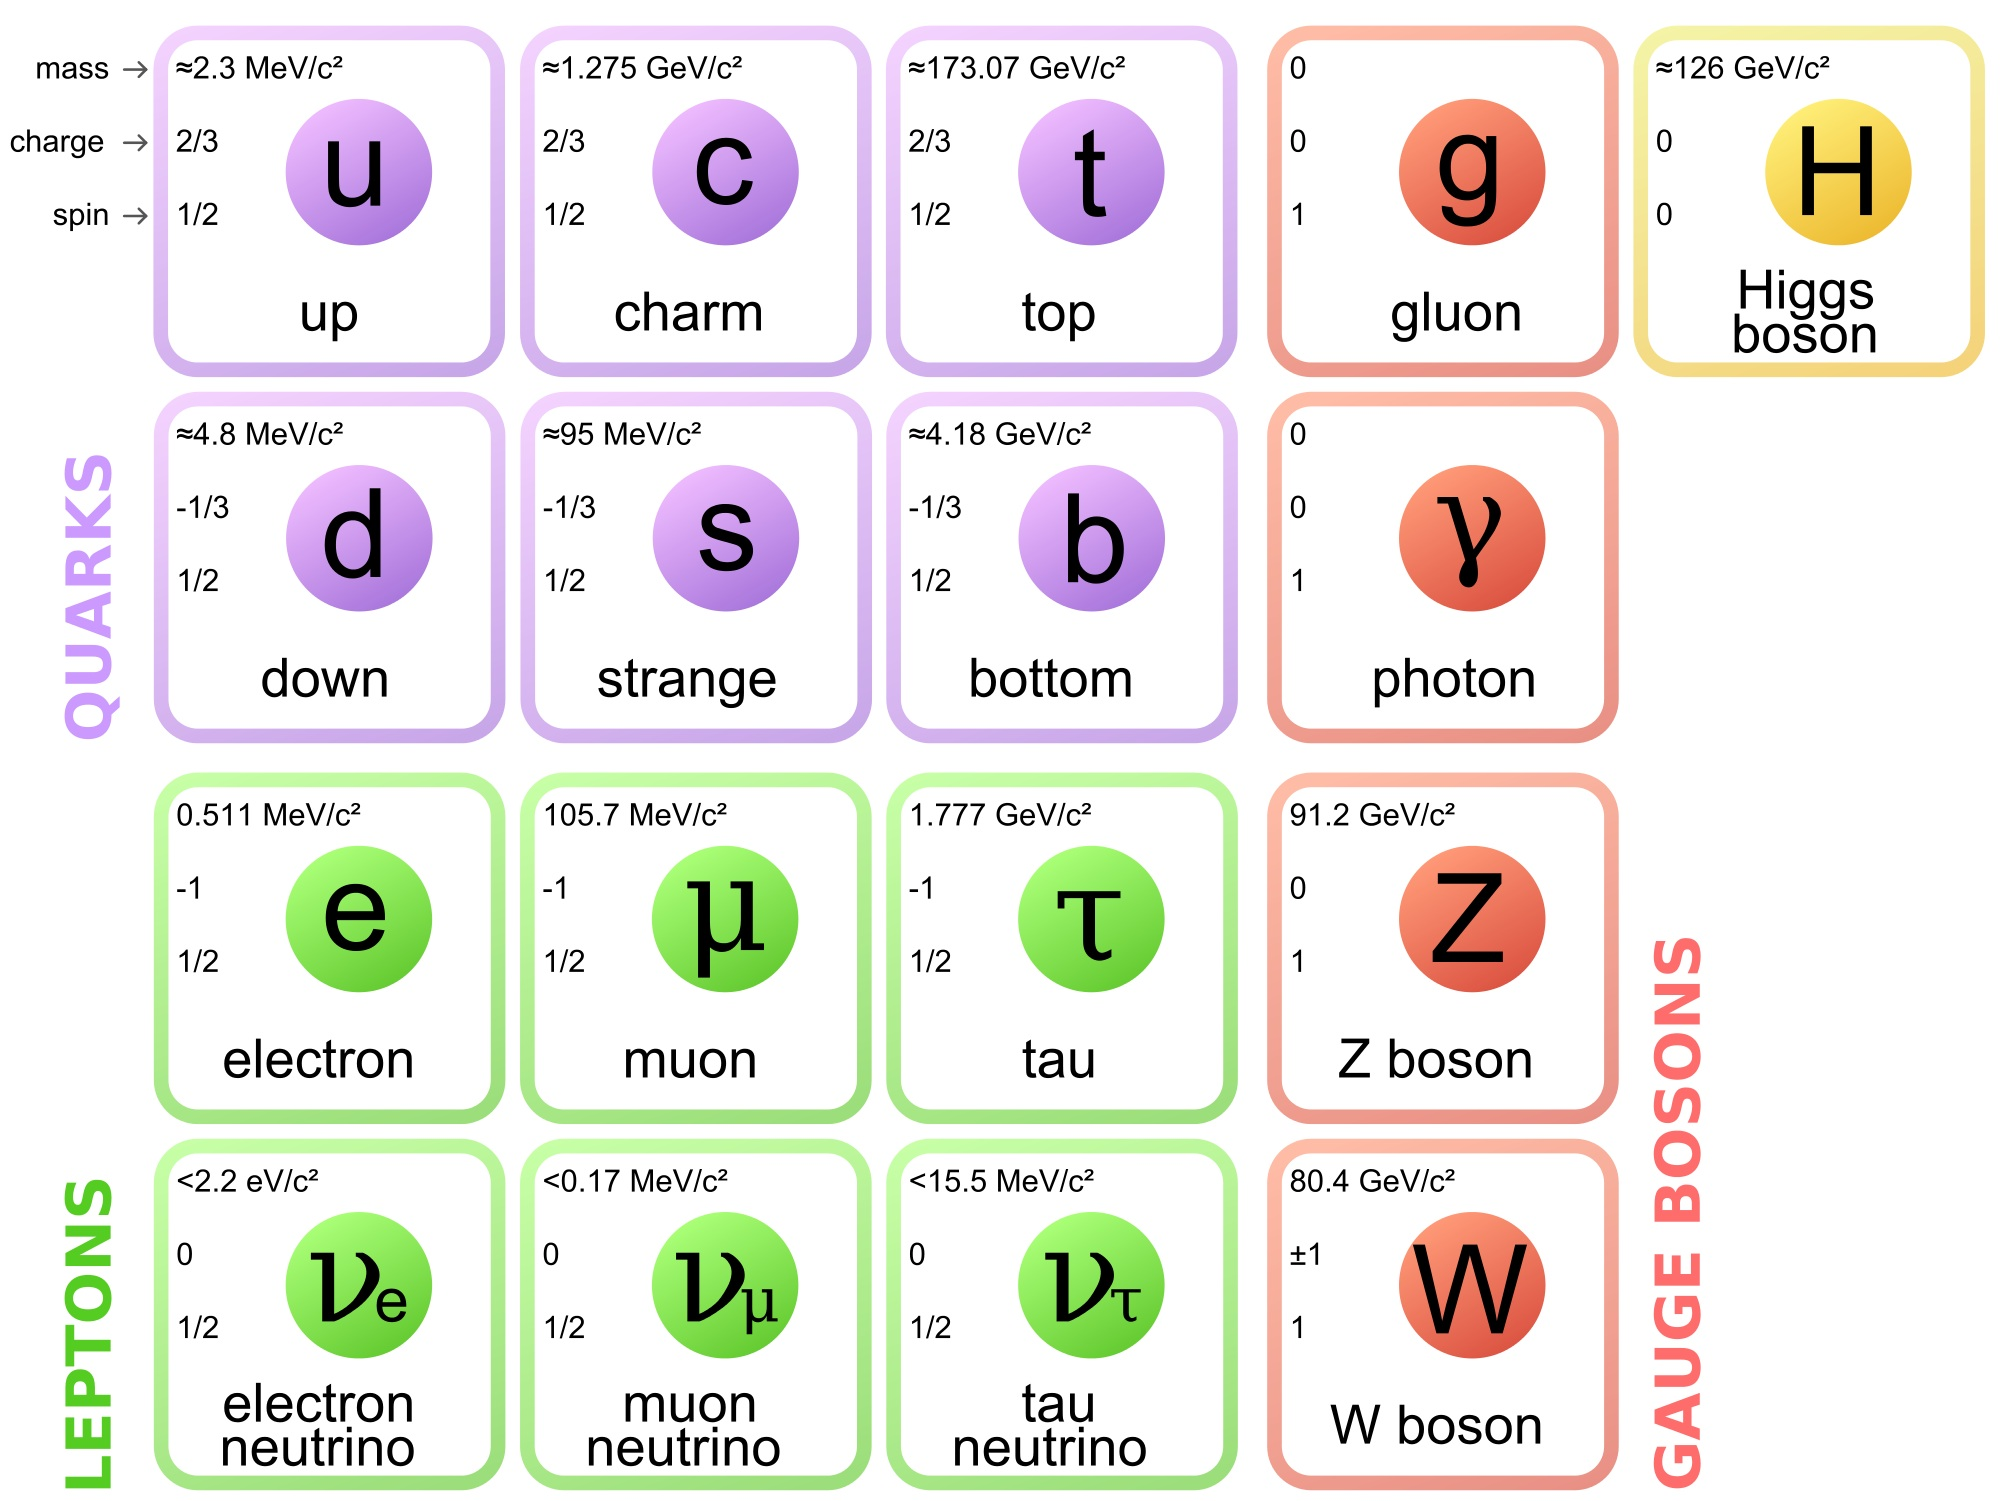
\includegraphics[width=0.8\linewidth]{figures/StandardModel.jpg}
    \caption{Particles in the SM}
    \label{fig:SM}
\end{figure}
The Standard Model of particles (SM) is the most currently utilized theory of interactions of subatomic particles. It describes all 
matter particles and forces between them, excluding gravity, as interactions between 12 fermions (6 quarks and 6 leptons) with their corresponding anti-fermions, 4 spin-1 force-carrying gauge bosons and 1 scalar boson as shown in Fig. \ref{fig:SM}. Within this framework exist 3 distinct forces: strong nuclear force, mediated by the gluon ($g$) boson; electromagnetic (EM) force, mediated by the photon ($\gamma$) boson; and weak nuclear force, mediated by the $W^{\pm}$ and $Z$ bosons. 
This work pertains to the description of the properties of the only family of particles that present no electric or color charge known as neutrinos ($\nu$), wherein the SM exist three known flavors ($\nu_e$, $\nu_\mu$ and $\nu_\tau$) corresponding to the latter half of (electro)weak isospin doublets formed with the known charged leptons ($e^-$, $\mu^-$ and $\tau^-$). This chapter aims to describe neutrinos in the SM, the weak force and its origin as a part of a larger broken symmetry known as "Electroweak Theory" (EW). 
\section{Symmetries and fermion content}
\subsection{Neutrinos}
Neutrinos are charge-less, color-less, spin-$\frac{1}{2}$ particles with negligible masses compared to other fundamental particles first proposed in 1930 by Pauli W.~\cite{pauli1930neutrino}, and later detected by C. L. Cowan et al. in 1956~\cite{doi:10.1126/science.124.3212.103}, to solve known apparent contradictions in conserved quantities of beta decays. Beta decay was known to be as the emission of beta particles (electrons) by the nuclei of unstable atoms, wherein the difference in mass of the original and resulting nuclei of the decay should fix the energy at which the emitted particles are detected. Also of note, due to conservation of angular momentum the sum of the spin ($S_e$) of the electron, the spin of the resulting nucleus ($S_{N^{*}}$) and the angular momentum between them ($L$) should equal the original nucleus' spin ($S_{N}$). Despite this, it was know experimentally that the resulting electrons where emitted in a spectrum of energies less than expected and at $L=0$, making the sum of spins impossible to match.
Pauli's solution to the apparent violation of the conservation of these quantities was to hypothesize the existence of a second neutral spin-$\frac{1}{2}$ with very small mass compared to the electron that allows for both the distribution of energy between both emitted particle, thus letting the electron be emitted at different energies depending on the kinematics, and the conservation of angular momentum. 
\begin{align*}
    N &\rightarrow N^{*} + e^{-}     ~ &\rightarrow&    &N \rightarrow& N^{*} + e^{-} + \nu \\ \hline
    m_N &= m_{N^*} + E_{e^-}         ~ &\rightarrow&   &m_N =& m_{N^*} + E_{e^-} + E_{\nu} \\
    S_{z~N} &= S_{z~N^*} + S_{z~e^-} ~ &\rightarrow&   &S_{z~N} =& S_{z~N^*} + S_{z~e^-} + S_{z~\nu}
\end{align*}
Later refinement of the atomic model found that nuclei where made up of positively charged elements named protons ($p$) and neutrally charged elements known as neutrons\footnote{this was the name first proposed for the particle hypothesized by Pauli, later changed} ($n$), leaving the small hypothesized particle to be named neutrino ($\nu$) later by Enrico Fermi. It is well understood now that the beta decay is a process in which a neutron within an unstable nucleus decays into a proton, an electron and a(n) (anti)neutrino.  
$$n \rightarrow p + e^{-} + \bar{\nu}$$
Subsequent experiments exploiting cross symmetry of the above interaction~\cite{doi:10.1126/science.124.3212.103}, accelerator-produced pion decay~\cite{Danby1962}, and charged-current tau neutrino interactions in nuclear emulsion~\cite{Kodama2001, Kodama2008} confirmed the existence of three distinct active neutrino flavors and the conservation of lepton family number in the interactions that involved these particles. Given that neutrinos don't interact via electromagnetic or strong forces a theory of a different force that mediated these interactions was developed into what is now known as the "weak nuclear force".
\subsection{Weak Nuclear Force}
Developments in quantum mechanics (QM) and special relativity (SR) led up to the first theories that could describe the behavior of some subatomic particles and their interactions through excitations of quantized fields called quantum field theories (QFTs) obtained by promoting classical fields to operator-valued quantities satisfying canonical (anti)commutation relations and deriving their dynamics from a Lorentz-invariant action principle. One of the earliest and most successful QFTs was Quantum Electro Dynamics (QED), describing how spin-1/2 (anti)particles (\stackon[.1pt]{$\psi$}{\brabar}) interacted with an EM 4-potential ($A^\mu$) by minimizing the action given by the lagrangian density: 
\begin{equation}
    \mathcal{L}_{\text{QED}} = \underbrace{\bar{\psi}(i\gamma^\mu\partial_\mu - m)\psi}_{\text{free Dirac field}} - \underbrace{\frac{1}{4}F_{\mu\nu}F^{\mu\nu}}_{\text{free EM field}} - \underbrace{e\bar{\psi}\gamma^\mu\psi A_\mu}_{\text{interaction}}.
    \label{eq:L_QED}
\end{equation}
While the `free' terms in (\ref{eq:L_QED}) describe the propagation of Dirac fermions and photons in free Minkowski space, the `interaction' term describes a vertex that couples the (anti)fermion current with the electromagnetic four-potential, representing the elementary process of a(n) (anti)fermion emitting or absorbing a photon. At zeroth-order $\hbar$ perturbative terms, QED had shown predictive power for processes like Compton ($\gamma + e^- \rightarrow \gamma + e^-$)~\cite{KleinNishina1929} and M\o ller ($e^- + e^- \rightarrow e^- + e^-$)~\cite{Moller1932} scattering by the time Fermi first proposed an interaction inspired by the QED interaction term, where instead of a fermion current emits a photon, two fermion currents meet at a vertex such that a coupling constant (now called Fermi's constant $G_F$) quantified the intensity of the interaction, and thus can be estimated experimentally.
\begin{center}
% https://feynman.srossd.com/#N4Igdg9gJgpgziAXAbVABwnAlgFyxMJZABgBoBGAXVJADcBDAGwFcYkQQBfU9TXfQinIVqdJq3ZceIDNjwEiAJlLFRDFm0QduvOQKWlFa8Zu3TZ-BSmVUa6iVoC8U3ZcHIAzCLsn2AHT9sAFsXGT55dzIAFmMNSR0wvStkYRi7GAAnHBgAD3YoCBxQiwiDD1iHM1dS61I0sTitYvD9WoBWCtNmpPcvevtTAODutyIo7wbKmACAI3oM4AC0bE4AfWAAM04AgHN6IKD6AD0AoOYl7HWtgAIAQVXT5hGa5HH+3y0AgAoAjYz6ADGwAA4qsAGKcRaBACOWWAik4nB+fjmCwuWDWwDA2z8ewOx0e6PWaE4AEpkaiocsMesAmBmDi8YcHn4zkTgDAjsAALSI0kBUnPVokFRqTLZPJaApFBIlYVtOqdfx+P6AkHgyFDWE4eGIinzKkrdbY3b7Q4nVnnPzU4lk-Vo61GqH0xlm+gstmOrDrTk8vlC5IK2yTUzTFEG9GYram-EWz02zacO4ep6cUQwKA7eBEUB-CAhRBkEA4CBIYQgAEAC3mWbLNEY9BmMEYAAUWlYQIwYBsij5GiANqE8wXyyWkMoK9WMrXEOXGFgwKYNpkgvo+5VBwlh3Xi6XEF5OwvTGhK4UFPXG822z12BksDtK72Q8qmfQhxl80gAGw0MeIADsNBVjWmjlgM7BoO+n6IAAHL+e6AZOIFINyYEfOAUEFgAnPBSCIcB06geugzhg6LqYWWRZ-vhU4zqhxHsJy3JcJQnBAA
\begin{tikzpicture}
\begin{feynman}
\vertex (0) at (0, 8);
\vertex (1) at (2, 8);
\vertex (2) at (4, 10);
\vertex (3) at (4, 6);
\vertex (4) at (4, 8);
\vertex (5) at (6, 8) {\(\sim\)};
\vertex (6) at (0, 2);
\node[dot] (7) at (2, 2);
\vertex (8) at (4, 4);
\vertex (9) at (4, 2);
\vertex (10) at (4, 0);
\vertex (11) at (6, 2) {\(\sim\)};
\vertex (12) at (8, 8) {\(e\bar{\psi}_{f}\gamma^\mu\psi_{f} A_\mu\)};
\vertex (13) at (8, 2);
\vertex (18) at (10, 2) {\(\mkern-80mu \frac{G_F}{\sqrt{2}}(\bar{\psi}_{n}\gamma^\mu\psi_{p})(\bar{\psi}_{\nu}\gamma_\mu\psi_{e^{-}})\)};
\vertex (19) at (10, 8);
\diagram*{
	(0) --[fermion,edge label={\(f\)}] (1),
	(1) --[fermion,edge label={\(f\)}] (2),
	(1) --[photon,edge label'={\(\gamma\)}] (3),
	(6) --[fermion,edge label={\(p\)}] (7),
	(8) --[anti fermion,edge label={\(n\)}] (7),
	(9) --[fermion,edge label={\(\bar{\nu}\)}] (7),
	(10) --[anti fermion,edge label={\(e^-\)}] (7)
};
\end{feynman}
\end{tikzpicture}
\end{center}
Subsequent discoveries in particle physics revealed that charged-current weak interactions violate parity symmetry maximally. First theorized by Lee and Yang in 1956~\cite{Lee:1956qn} to resolve the then-known $\tau - \theta$ puzzle, and later verified experimentally by Wu et al. in 1957~\cite{Wu:1957my}, this motivated a modification of the Fermi interaction in the form of a combination of the two bilinear Lorentz-invariant structures that admit such violation~\cite{Sudarshan:1958vf, Feynman:1958ty}.

\begin{align}
\text{V}&:  j_{V}^{\mu} = \bar{\psi}\gamma^\mu\psi &\xrightarrow{\mathcal{P}}& &j'_{V~\mu} &= \bar{\psi}\gamma_\mu\psi& \label{eq:V}\\
\text{A}&:  j_{A}^{\mu} = \bar{\psi}\gamma^\mu\gamma^5\psi &\xrightarrow{\mathcal{P}}& &j'_{A~\mu} &= -\bar{\psi}\gamma_\mu\gamma^5\psi& \label{eq:A}
\end{align}

The expressions (\ref{eq:V}) and (\ref{eq:A}) show how different bilinear structures change under parity ($\mathcal{P}$) and how pure vector (axial) currents are $\mathcal{P}-even$ ($\mathcal{P}-odd$). Given a general current structure, $j^\mu = g_V j_{V}^\mu + g_A j_{A}^\mu$, observables that depend on the inner product of two such currents transform under parity as:
\begin{align}
    |\mathcal{M}|^2 &= (j_{1} \cdot j_{2}) = g_V^2 (j_{1~V} \cdot j_{2~V}) + g_A^2 (j_{1~A} \cdot j_{2~A}) + g_V g_A (j_{1~V} \cdot j_{2~A} + j_{1~A} \cdot j_{2~V})\label{eq:M} \\  \nonumber
    &\xrightarrow{\mathcal{P}} \\
    |\mathcal{M}'|^2 &= (j'_{1} \cdot j'_{2}) = g_V^2 (j'_{1~V} \cdot j'_{2~V}) + g_A^2 (j'_{1~A} \cdot j'_{2~A}) - g_V g_A (j'_{1~V} \cdot j'_{2~A} + j'_{1~A} \cdot j'_{2~V}).\label{eq:Mprime}
\end{align}
The only difference between \ref{eq:M} and \ref{eq:Mprime} lies in the sign of the interference term, such that the degree of $\mathcal{P}$-symmetry violation is given by the coefficient $\frac{g_V g_A}{g_V^2 + g_A^2}$. Normalizing this there are two options for maximally violated $\mathcal{P}$-symmetry given by $\frac{g_V}{g_A} = \pm 1$, also known as $V\pm A$ currents. Given that in the Wu experiment it was determined that (anti)neutrinos are emitted exclusively as left(right)-handed fermions the appropriate structure to use for weak interactions was determined to be $V-A$. Modifying the Fermi lagrangian density for beta decay to include this gives the following expression:
\begin{equation}
    \mathcal{L}_{CC}=\frac{G_{F}}{\sqrt{2}}\left[\bar{\psi}_{\nu_{e}}\gamma^{\mu}(1-\gamma^{5})\psi_{e}\right]\left[\bar{\psi}_{p}\gamma_{\mu}(1-\gamma^{5})\psi_{n}\right]+\text{h.c.} \label{eq:VALag}
\end{equation}
Later refinements of this theory succeeded in demonstrating the universality of the weak interaction across leptonic decays and strangeness-changing meson decays through Cabibbo mixing~\cite{Cabibbo:1963yz}. This not only established that all such processes are mediated by the same underlying force, but also motivated the prediction and subsequent discovery of the charm quark~\cite{Glashow:1970gm}. With these improvements on the theory thus far, the point-like structure of the interaction still led to scattering amplitudes proportional to the center-of-mass energy $\sqrt{s}$, resulting in S-matrix unitarity violation at higher energies. The natural resolution, in analogy with QED, is to conceive of Fermi's interaction as the low-energy limit of a gauge field theory, wherein the maximal parity violation of the charged currents naturally gives rise to three mediating vector bosons corresponding to the generators of an $SU(2)_L$ symmetry, which must be massive due to the short range of the weak interaction. Given this hypothesis, Glashow showed in 1961~\cite{Glashow1961} that the gauge field theory whose low-energy limit reproduces the $V-A$ structure of charged currents requires a $SU(2)_L \times U(1)_Y$ symmetry group, which not only predicted the existence of neutral weak currents, later measured in 1973 at the GARGAMELLE experiment at CERN~\cite{Hasert1973a, Hasert1973b},  but also unified the weak and electromagnetic interactions into a single electroweak theory, later developed independently by Weinberg and Salam~\cite{Weinberg1967, Salam1968}.
\section{Massive and Massless Mediators}

\section{Electroweak mixing $\sin^2 \theta_W$}


